\documentclass[a4paper,12pt]{article}
\usepackage{graphicx}

\usepackage[hidelinks=true, bookmarks=true]{hyperref}
\usepackage{epstopdf}
\usepackage{gensymb}
\usepackage{float}
\usepackage{mathtools}
\usepackage{setspace}
\usepackage{tabularx}
\usepackage{appendix}
\usepackage{svg}


\title{Kandidatprojektsrapport}
%% Definitioner för LIPS-dokument

\usepackage[swedish]{babel}
\usepackage[utf8]{inputenc}
\usepackage[T1]{fontenc}
\usepackage{times}
\usepackage{ifthen}
\usepackage[labelfont=it]{caption}

\usepackage[margin=25mm]{geometry}

\def\arraystretch{1.6}

\usepackage{fancyhdr}
\pagestyle{fancy}
\lhead{}
\chead{\LIPSprojekttitel}
\rhead{\LIPSdatum}
\lfoot{\LIPSkursnamn \\ \LIPSdokumentansvarig}
\rfoot{\LIPSprojektgrupp \\ \LIPSgruppepost}

\setlength{\parindent}{0pt}
\setlength{\parskip}{1ex plus 0.5ex minus 0.2ex}


\newcommand{\twodigit}[1]{\ifthenelse{#1<10}{0}{}{#1}}
\newcommand{\dagensdatum}{\number\year-\twodigit{\number\month}-\twodigit{\number\day}}

%% ------------------------------------------
% NYBILD
% Skapar centrerad bild med caption
%   
% #1: Filens url relativt '/bilder/'
% #2:  Caption
% #3: Label
% #4: Skalning i förhållande till textwidth
%% ------------------------------------------
\newcommand{\nyBild}[4] 
{\begin{figure}[H]
  \centering
 \emph{\includegraphics[angle=0,width=#4\textwidth]{bilder/#1}}
  \caption{\emph{#2}}
  \label{fig:#3}
\end{figure}}

%%  Redefinitions of commands containing @
\makeatletter
\makeatother

\newcommand{\LIPStitelsida}{%
{\ }\vspace{45mm}
\begin{center}
  \textbf{\Huge {\sffamily \LIPSdokumenttyp}}
\end{center}
\begin{center}
  {\Large \LIPSredaktor}
\end{center}
%\begin{center}
%  {\Large Version \LIPSversion}
%\end{center}
\vspace{60mm}
%\begin{center}
%  {\large Status}\\[1.5ex]
%  \begin{tabular}{|*{3}{p{40mm}|}}
%    \hline
%    Granskad & \LIPSgranskare & \LIPSgranskatdatum \\
%    \hline
%    Godkänd & \LIPSgodkannare & \LIPSgodkantdatum \\
%    \hline
%  \end{tabular}
%\end{center}
\newpage
}


\newenvironment{LIPSprojektidentitet}{%
{\ }\vspace{45mm}
\begin{center}
  {\Large PROJEKTIDENTITET}\\[0.5ex]
  {\small
  \LIPSprojektgrupp, \LIPSartaltermin, \LIPSprojekttitel\\
  Tekniska högskolan vid Linköpings universitet, ISY
  }
\end{center}
\begin{center}
  \begin{tabular}{|l|p{45mm}|p{25mm}|l|}
    \hline
    \textbf{Namn} & \textbf{Ansvar} & \textbf{Telefon} & \textbf{E-post} \\
    \hline
}
{
    \hline
  \end{tabular}
\end{center}
\begin{center}
  {\small
    \textbf{E-postlista för hela gruppen}: \LIPSgruppepost\\
    \textbf{Kontaktperson hos kund}: \LIPSkundkontakt\\
    \textbf{Kursansvarig}: \LIPSkursansvarig\\
    \textbf{Handledare}: \LIPShandledare\\
  }
\end{center}
\newpage
}
\newcommand{\LIPSgruppmedlem}[4]{\hline {#1} & {#2} & {#3} & {#4} \\}



\newenvironment{LIPSdokumenthistorik}{%
\begin{center}
  Dokumenthistorik\\[1ex]
  \begin{small}
    \begin{tabular}{|l|l|p{60mm}|l|l|}
      \hline
      \textbf{Version} & \textbf{Datum} & \textbf{Utförda förändringar} & \textbf{Utförda av} & \textbf{Granskad} \\
      }%
    {%
      \hline
    \end{tabular}
  \end{small}
\end{center}
}
\newcommand{\LIPSversionsinfo}[5]{\hline {#1} & {#2} & {#3} & {#4} & {#5} \\}



\newenvironment{packed_itemize}{
\begin{itemize}
	\setlength{\itemsep}{1pt}
    \setlength{\parskip}{0pt}
    \setlength{\parsep}{0pt}
}{\end{itemize}}

\newenvironment{packed_enumerate}{
\begin{enumerate}
	\setlength{\itemsep}{1pt}
    \setlength{\parskip}{0pt}
    \setlength{\parsep}{0pt}
}{\end{enumerate}}





%%% Local Variables: 
%%% mode: latex
%%% TeX-master: "kravspec_mall"
%%% End:

\usepackage{sectsty}
\allsectionsfont{\sffamily}

\usepackage{titlesec}
\titlespacing{\section}{0pt}{30pt}{10pt}
\frenchspacing


\renewcommand{\thepage}{\roman{page}}

\newcommand{\LIPSartaltermin}{VT14}
\newcommand{\LIPSkursnamn}{TSEA56 Elektronik kandidatprojekt}

\newcommand{\LIPSprojekttitel}{Lagerrobot}

\newcommand{\LIPSprojektgrupp}{Grupp 1}
\newcommand{\LIPSgruppepost}{tsea56-2014-grupp-1@googlegroups.com}
\newcommand{\LIPSdokumentansvarig}{Kandidatrapport}

\newcommand{\LIPSkund}{ISY, Linköpings universitet, 581\,83 Linköping}
\newcommand{\LIPSkundkontakt}{Tomas Svensson, 013-28 13 68, tomass@isy.liu.se}
\newcommand{\LIPSkursansvarig}{Tomas Svensson, 013-28 13 68, 3B:528, tomass@isy.liu.se}
\newcommand{\LIPShandledare}{Anders Nilsson, 3B:512, 013-28 26 35, anders.p.nilsson@liu.se}


\newcommand{\LIPSdokumenttyp}{Lagerrobot 

 \Large{Kandidatprojekt i elektronik}}
\newcommand{\LIPSredaktor}{Johan Lind 

Karl Linderhed 

Lucas Nilsson 

Philip Nilsson 

Patrik Nyberg 

Erik Nybom 

Andreas Runfalk 

}

\newcommand{\LIPSversion}{1.0}
\newcommand{\LIPSdatum}{\dagensdatum}

\newcommand{\LIPSgranskare}{}
\newcommand{\LIPSgranskatdatum}{}
\newcommand{\LIPSgodkannare}{}
\newcommand{\LIPSgodkantdatum}{}

\begin{document}

\LIPStitelsida

%% Argument till \LIPSgruppmedlem: namn, roll i gruppen, telefonnummer, epost
\begin{LIPSprojektidentitet}
  \LIPSgruppmedlem{Karl Linderhed}{Projektledare (PL)}{073-679 59 59}{karli315@student.liu.se}
  \LIPSgruppmedlem{Patrik Nyberg}{Dokumentansvarig (DOK)}{073 -049 59 90}{patny205@student.liu.se}
  \LIPSgruppmedlem{Johan Lind}{}{070-897 58 24}{johli887@student.liu.se}
  \LIPSgruppmedlem{Erik Nybom}{}{070-022 47 85}{eriny778@student.liu.se}
  \LIPSgruppmedlem{Andreas Runfalk}{}{070-564 23 79}{andru411@student.liu.se}
  \LIPSgruppmedlem{Philip Nilsson}{}{073-528 48 86}{phini326@student.liu.se}
  \LIPSgruppmedlem{Lucas Nilsson}{}{073-059 42 94}{lucni395@student.liu.se}
\end{LIPSprojektidentitet}


\renewcommand*\contentsname{Innehåll}
\begin{spacing}{0.5}
\tableofcontents{}
\end{spacing}
\newpage

%% Argument till \LIPSversionsinfo: versionsnummer, datum, ändringar, utfört av, granskat av
%\addcontentsline{toc}{section}{Dokumenthistorik}
\begin{LIPSdokumenthistorik}
  \LIPSversionsinfo{1.0}{2014-05-21}{Ursprunglig version}{EN}{Alla gruppmedlemmar}
\end{LIPSdokumenthistorik}
\newpage

\renewcommand{\thepage}{\arabic{page}}
\setcounter{page}{1}

\newpage


\section{Inledning}
Sju studenter vid Linköpings Universitet valde i deras kandidatprojektkurs TSEA56 att konstruera en automatiserad lagerrobot utifrån beställarens krav på design och funktion. Projektet gjordes med avsikten att ge studenterna bildning och erfarenhet att med de kunskaper erhållna från tidigare kurser kunna genomföra ett omfattande uppdrag med samma metodik som förekommer i arbetslivet.

Produkten är en lagerrobot på fyra hjul med en robotarm monterad ovanpå. En linjesensor framtill används för att roboten ska kunna följa en linje bestående av svart tejp, detektera plock- och avlämningsstationer, hantera avbrott i tejpen samt hantera korsningar. Vid plockstationer söker roboten efter föremål med hjälp av en sidoskanner. Vid objektidentifiering beräknas en koordinat som armen använder sig av för att med hjälp av inverterad kinematik förflytta sig till föremålet autonomt. Roboten kan även styras manuellt i ett datorgränssnitt via blåtandskommunikation. 

Projektgruppen fick robotikhårdvaran (hjulbasen med strömförsörjning och robotarmen) färdigbyggd från beställaren. Projektuppgiften bestod i att designa och utveckla kretskort med mikroprocessorer, elektronik och sensorer för att klara av ett givet uppdrag. 


\section{Problemformulering}

För att roboten ska kunna navigera genom lagerutrymmet finns det en bana markerad med svart tejp på golvet. Längs med tejpen markeras de stationer där föremål ska plockas upp respektive lämnas av med hjälp av en bit tejp vinkelrät mot banan.

\nyBild{bana.pdf}{Översiktlig bild av bana och robot}{bana}{0.75}

Roboten måste även kunna avgöra om ett föremål ska plockas upp på en station och på vilken station föremålet ska lämnas av. Därför är stationerna utrustade med var sin RFID-tagg\footnote{RFID (Radio Frequency Identification) är en teknik som kan användas för trådlös identifiering. Olika varianter finns, men i projektet används en aktiv läsare som identifierar passiva taggar.} innehållandes ett för stationen unikt identifikationsnummer. För detaljer, se banspecifikationen i bilaga \ref{sec:banspec}.

De grundläggande krav roboten måste uppfylla för att klara uppgiften inkluderar att följa en linje, läsa av RFID-taggar samt att plocka upp föremål. Utöver dessa grundläggande krav är projektets tillämpbarhet på ett verkligt scenario i stor del beroende av att kraven inte bara kan uppfyllas, utan även utföras autonomt. Av denna anledning så innefattar den utökade kravbilden, i kravspecifikationen markerad med lägre prioritet, i huvudsak krav vilka innebär en för roboten ökad autonomi.

En ökad grad av autonomi innebär i detta projekt huvudsakligen att roboten klarar av att plocka upp samt sätta ned föremål utan mänsklig inblandning. Detta medför att uppgiftens komplexitet snabbt ökar då kravbilden utökas förbi den grundläggande funktionalitet som i kravspecifikationen är beskriven med prioritet 1. Robotens förmåga att plocka upp ett föremål autonomt kräver inte bara förmågan att kontrollera armen, utan även ett system för att insamla information om föremålets exakta position samt att översätta och vidarebefordra denna information till armen. Vidare måste armen i sin tur kunna röra sig i rummet med en sådan precision att upplockning av föremål kan göras utan att en människa kontinuerligt korrigerar armens position.




\section{Kunskapsbas}

Majoriteten av komponenterna som använts i projektet finns dokumenterade med datablad och förklaringar på ISY:s (Institutionen för systemteknik vid Linköpings universitet) databladssida Vanheden \footnote{\url{https://docs.isy.liu.se/twiki/bin/view/VanHeden}} och det är i huvudsak därifrån som specifikationer och data har inhämtats. Där finns bland annat datablad för mikroprocessorn ATmega 1284P, som används för alla fyra delsystem i projektet. 

Kunskapen som varit nödvändig för att genomföra projektet har till största del tillkommit projektgruppen under deras tidigare studier där gruppmedlemmarna bland annat har lärt sig programmering och enklare elektronikkonstruktion. Vidare har de primära källorna för ytterligare information varit de datablad som finns på Vanheden, samt projektgruppens handledare vid ISY. 

I övrigt har de dokument som skapats i förstudien och uppstarten av projektet använts som stöd under det fortsatta arbetet. Projektets dokument beskrivs i avsnitt \ref{sec:utforande}. Särskilt har designspecifikationen legat till grund för allt det konstruktions- och programmeringsarbete som skett i projektet.
\input{Genomförande}

\section{Teknisk beskrivning}

Roboten är uppdelad i fyra olika delsystem med varsitt ansvarsområde som vart och ett löser ett tydligt delproblem. Det första av delsystemen, kallat chassit, kontrollerar motorer och har en regleralgoritm för att se till att roboten följer linjen. Denna enhet har även det övergripande ansvaret för roboten. Det betyder till exempel att den säger till delsystem arm då det är dags att plocka upp ett föremål. Detta innebär att den också ansvarar för att föremål ställs ned och plockas upp på rätt station.

Armenheten kontrollerar och styr de servon som sitter i robotarmen och ansvarar för funktionaliteten som krävs för att plocka upp samt sätta ner föremål vid plockstationerna.

Sensorenheten är den enhet som samlar in den information som resten av roboten använder för att ta de styrbeslut som krävs för att slutföra uppgiften. Denna enhet svarar bara på förfrågningar av andra enheter och tar inga egna initiativ för att börja samla information.

Kommunikationsenhetens uppgift är att kommunicera relevant information ut till omvärlden. Detta görs dels till datorn med hjälp av blåtand, dels med hjälp av en LCD-skärm monterad på roboten. Även denna fungerar som en slav och skriver endast saker på skärmen då någon säger åt den att göra det. Den vidarebefordrar också data mellan robotens delsystem och en persondator via bussen samt blåtand.

\nyBild{Robot_oversikt.png}{Översikt över robotens delar}{robotoversikt}{0.8}

%\begin{test}
%  \LIPSversionsinfo{0.1}{2014-05-20}{Första utkast.}{EN}{LN}
%\end{test}
%\newpage

Figur \ref{fig:robotoversikt} visar huvuddelarna på kretskorten med följande numrering:
\begin{packed_enumerate}
\item Strömbrytare till batteriet
\item Sensorenhetens processor
\item Knapp för nollställning av sensorenhet
\item Blåtandsmodem för kommunikation mellan robot och persondator
\item Kommunikationsenhetens processor
\item Armenhetens processor
\item Knapp för nollställning av kommunikationsenhetens och armenhetens processorer
\item Knapp för att påbörja linjeföljning i autonomt läge
\item Knapp för nollställning av chassienhetens processor
\item Chassienhetens processor
\item Omkopplare för val av autonomt eller manuellt läge
\end{packed_enumerate}




\section{Chassi}

Chassienheten är den enhet som styr över de andra enheterna och bestämmer när de andra enheterna ska utföra sina uppgifter. Chassit är också den enhet som styr motorerna till hjulen. Motorerna är kopplade så att både fram och bakhjul på vardera sida får samma styrsignal, så styrningen blir liknande den på en bandvagn. Motorerna styrs genom en PWM-signal som skickas från chassienhetens processor, se bilaga XX. Till chassienheten finns även en omkopplare där man kan välja mellan att roboten ska följa linjen autonomt eller om den bara ska gå att styra via persondatorn. Det finns även en tryckknapp som används för att påbörja linjeföljningsproceduren.

\nyBild{chassi_huvudprogram.pdf}{Översiktlig bild av Chassits huvudprogram}{huvudprogram}{0.7}

Chassits huvudprogram startas genom ett knapptryck eller via ett kommando från persondatorn. Då säger chassit till sensorenheten att börja söka efter en linje att följa. Ifall omkopplaren står på manuellt läge händer ingenting mer. Annars ber chassit sensprenheten med jämna mellanrum om en tyngdpunkt samt information om ifall roboten har en station till höger eller vänster. Detta görs fram tills dess att sensoreneheten skickar att roboten är på station. Med hjälp av tyngdpunkten och PD-reglering beräknar chassit vilken hastighet hjulen på vardera sida ska ha för att det ska bli en mjuk lineföljning, se bilaga XX. 

När sensorenheten skickar att den har upptäckt en station stannar roboten. Sedan säger chassit till sensorenheten att läsa in RFID-taggen som förhoppningsvis ligger under roboten. Sensorenheten skickar tillbaka vilket värde RFID-taggen har. Ifall ingen tagg hittas kör roboten lite framåt och ber sensorenheten att göra en ny läsning. Hittas ingen tagg efter att roboten kört både framåt och bakåt en bit ger roboten upp och kör vidare till nästa station. Om det däremot hittas en tagg tar chassienheten beslut om vad som ska göras beroende på vilket ID taggen har. Beslutet beror på ifall det är en upplockningsstation eller avlämningsstation samt ifall roboten redan bär på något eller ifall stationen redan är avklarad. 

Om roboten har stannat på en station där ett föremål ska plockas upp skickar chassit ett kommando till armen som talar om att ett objekt ska plockas upp och på vilken sida av roboten föremålet befinner sig. När armen sedan utfört sin uppgift enligt kommandot från chassit skickar armen tillbaka att den är klar och om den klarade av att plocka upp eller lägga ner objektet. 

Roboten håller reda på huruvida alla stationer är avklarade genom att räkna hur många stationer den passerar innan den når samma station igen. När alla stationer är avklarade står roboten kvar på sista stationen och texten “Mission Complete” skrivs ut på LCD-displayen. Annars kör roboten vidare till nästa station. Vid varje beslutspunkt i chassits huvudprogram skickar chassit sitt beslut till kommunikationsenheten som i sin tur vidarebefodrar detta till den fjärranslutna datorn. De olika beslutspunkterna är som följer: stanna vid plockstation, RFID inläst, skickar kommando till arm samt arm är klar. 

\subsection{Arm}

Armen på roboten är av modell PhantomX Reactor från Trossen Robotics, med 7st AX-12A servon och 4st rörliga leder samt en gripklo. Servona skickar och tar emot data pararellt på samma kabel vilket gjorde att en tri-state buffer (fotnot: en krets som kan dela en kabel till en in- och en utport beroende på värdet på en enableport) varit nödvändig för programmet att kunna välja om den vill skicka till eller ta emot från servona. Servona kommunicerar med processorn genom USART. Varje servo har tar emot all data som skickas från processorn, men agerar endast på de kommandon som är riktade till dess eget unika ID.

Då kommandona som skickas är flera byte långa byggs dessa upp på förhand innan de skickas. Det är viktigt att det inte blir avbrott i kommunikationen för att processorn ska beräkna nästa byte. Om det inträffar skulle datan feltolkas och inte nå fram. Därför inaktiveras avbrott under själva överföringen. Vid varje sändning som riktas till ett enskilt servo fås ett svar tillbaka från med statuskod och eventuella parametrar. Detta svar används för eventuell felhantering. Eftersom gruppen valt att kunna styra robotarmen autonomt är det extra viktigt att kontrollera att varje instruktion blivit korrekt mottagen. Därför väntar programmet på svar från servona efter varje sändning gjorts. Dessa statuskoder kan sedan tolkas av programmet för att avgöra om kommandot nådde servot.

För ytterligare säkerhet gällande kommandon till servon, speciellt rörelser, har gruppen valt att endast sköta instruktioner genom funktionen reg-write som servona har. Med reg-write kan man ge ett servo en instruktion som endast utförs då ytterligare ett kommando, action-kommando, skickas till servot. Då all statusinformation finns tillgänglig kan programmet säkerställa att servona kommer agera som planerat innan rörelser utförs. Detta är väldigt användbart i de fall hela armen ska röras eftersom en led som inte rör sig kan ge en slutposition som i värsta fall skadar roboten.
Vid både manuell och autonom styrning av armen beräknas ledvinklar med inverterad kinematik (Metoden för inverterad kinematik beskrivs i bilaga \ref{sec:regleruppgift}). Armen kan styras manuellt i djupled, höjdled och rotation av basplatta. Gripklon kan öppnas och stängas manuellt. När armen rör sig manuellt räknas startpositionen ut och sedan adderas kontinuerligt önskad förändring så länge som armen förflyttas. Vid autonom rörelse får armenheten en vinkel och ett avstånd från basplattan till föremålet som ska plockas upp. Genom inverterad kinematik ställer armen in sig och greppar föremålet. Koordinaten som föremålet plockades upp på sparas ned och används vid avlämning för att garantera att föremålet inte ska falla omkull.

Huvudprogrammet för armenheten är passivt tills enheten anropas över bussen. Busskommandona sätter olika flaggor som huvudprogrammet kontinuerligt läser av.



\subsection{Sensor}

Sensorenheten har tre huvudsakliga uppgifter. Den är ansvarig för att ta fram data utifrån vilken roboten ska klara av att följa en linje samt hantera plockstationer. Vidare är dess uppgift att vid plockstationer tillhandahålla armenheten med koordinater till det objekt som ska plockas upp samt att läsa av RFID-taggarna som ligger på banan i samband med plockstationerna. Information om vilken RFID-tagg som ligger vid stationen vidarebefodras till chassienheten som utifrån detta avgör huruvida stationen i fråga är en plockstation eller avlämningsstation.

För att följa en linje krävs för det första att sensorenheten klarar av att detektera tejplinjen. Detta åstadkommes med hjälp av en reflexsensormodul beståendes av elva separata reflexsensorer. En reflexsensor är i sin tur uppbyggd av en infraröd diod samt en fotokänslig transistor. Reflexsensormodulen är monterad längst fram på roboten ett par millimeter över golvet. När den infraröda dioden på varje reflexsensor tänds kommer detta ljus att studsa mot underlaget och ge upphov till en ström i transistorn. Ju mer ljus som reflekteras av underlaget, ju större kommer denna ström att vara. På detta sätt kan man då beräkna en tyngpunkt som motsvarar där linjen bör vara.

Sensorenhetens uppgift i robotens linjeföljning är alltså att samla in och omvandla den data som fås från reflexsensormodulen på ett sådant sätt att chassienheten kan utnyttja denna för att styra roboten längs med linjen. Detta görs genom att koppla dioder respektive fototransistorer till två stycken multiplexrar. Dessa multiplexrar styrs av sensorenhetens processor och används för att genom en A/D-omvandlare ta in data från var och en av reflexsensorerna som sitter på reflexsensormodulen. Denna data lagras sedan i processorn som ett åtta bitar stort heltalsvärde. Det innebär att varje reflexsensor kommer att registrera ett värde mellan 0 och 255, där 255 betyder mörkt underlag och 0 innebär ljust underlag.

Utifrån den data som lagrats i sensorenhetens processor beräknas sedan en tyngdpunkt på samma sätt som en linjetyngdpunkt i mekanik kan beräknas. Reflexsensorn ses som en linje där varje reflexsensors värde motsvarar tyngden för det segment av linjen den sitter på. Den tyngdpunkt som beräknas skalas till ett värde mellan 0 och 255, där 0 innebär att linjen ligger längst till vänster på sensorn och 255 innebär att linjen ligger längst till höger. 

Sensorns andra uppgift, att lokalisera de objekt som ska plockas upp, görs med hjälp av två stycken sidoskannrar, en på höger respektive vänster sida av roboten. Varje sidoskanner består av ett servo av enklare modell på vilket en optisk avståndssensor sitter monterad. För att hitta objekt så stegas servot upp i små inkrement. Efter att servot har stegats upp läses avståndssensorn av. Ifall att avståndssensorn registrerar ett avstånd som är större än robotarmens räckvidd innebär detta att objektet inte finns i den aktuella vinkeln varpå servot stegas upp ytterligare.

När sidoskannern för första gången läser av ett avstånd som är mindre än robotarmens räckvidd innebär detta att ett objekt har detekteras. För att hitta objektets mittpunkt stegas nu servot upp ytterligare tills dess att ett avstånd som återigen är större än robotarmens räckvidd detekteras. Objektets mittpunkt ligger då i den vinkel och avstånd som är mitt emellan de vinklar där objektet först och sist upptäcktes. För att dessa värden ska kunna användas av armenheten måste de först omvandlas för att vara anpassade till armens koordinatsystem som har sin nollpunkt i mitten av roboten, och inte ute på sidan där sidoskannrarna sitter. Exakt hur detta görs finns ingående beskrivet i den tekniska dokumentationen, se bilaga \ref{sec:tekdok}.

RFID-inläsningen görs genom att RFID-läsaren aktiveras och efter cirka 150 ms skickar den ett 12 bytes långt inläst ID via USART till processorn som lagrar detta värde i en buffert. Värdet i bufferten läses av och jämförs mot de ID:n som redan finns lagrade i processorns minne. Då en träff på ett av de lagrade ID:na sker med det inlästa skickas den siffra som står på RFID-taggen till chassit. 







\subsection{Kommunikation}

Kommunikationsenhetens uppgift är att förmedla data mellan robot, dator och omgivningen. Detta sköts dels via den skärm som finns på roboten och dels via det blåtandsmodem som sitter monterat på roboten. Skärmen har främst använts till att felsöka roboten under utvecklingsarbetet. I den färdiga produkten har datorn istället tagit över en stor del av skärmens informationsförmedlande uppgift. Skärmen ger dock även i robotens slutgiltiga utförande information om plockstationer samt RFID-taggarnas värde.

För att styra roboten finns ett program för en persondator där olika kommandon kan skickas till roboten. Från denna kan hjulen styras med antingen musklick eller tangentbord och det går även att starta eller stoppa linjeföljning och sätta nya parametrar till regleringen. Vidare finns möjligheten att styra armen, antingen manuellt eller genom att aktivera förprogrammerade rörelser.

I datorgränssnittet presenteras även information som skickas från roboten. De styrbeslut som roboten tar under autonom körning presenteras i gränssnittets loggfönster och den från linjesensorn beräknade tyngdpunkten plottas i en realtidsgraf. Vidare presenteras de avstånd som fås in från sidoskannrarna i ytterligare en graf. Datan presenteras endast då den är relevant. Detta innebär att man exempelvis inte får någon graf över tyngdpunkten då roboten står vid en plockstation och inte heller någon data från sidoskannrarna då roboten rör sig mellan plockstationer.





\input{Fördjupningsuppgifter.tex}

\section{Resultat}

Projektgruppen har under projektets gång visat att en robot så som beskriven i den tekniska dokumentationen skulle vara ett fullvärdigt alternativ att användas i ett faktiskt lager. Detta har visats i de tester som utförts där roboten uppfyller alla krav med prioritet ett med god repeterbarhet. De tester som genomförts har i huvudsak bestått av att låta roboten plocka upp och sätta ner objekt medan den har följt banan. För att säkerställa robotens förmåga att konsekvent uppfylla kraven har den testats på en rad olika banor designade för att tänja på de gränser som finns uppsatta i banspecifikationen, bilaga \ref{sec:banspec}. Objekten har placerats i olika vinklar och på olika avstånd för att testa sidoskannrar och armenheten. Avbrott i tejpen, kurvradie samt korsningar har hanterats i olika situationer ett stort antal gånger.

Vidare har robotens kapacitet för att helt autonomt plocka upp och sätta ner föremål enligt de RFID-taggar som ligger utlagda vid plockstationerna. All relevant sensordata vidarebefordras även till en persondator vilket möjliggör övervakning av roboten utan behov av direkt kontakt mellan människa och robot. Att roboten är autonom gör även att den är väldigt enkel att använda eftersom den efter uppstart inte kräver någon vidare mänsklig inblandning.


\section{Slutsatser}

Gruppen har under projektet dragit stor nytta av det grundliga arbete som gjordes i designspecifikationen. Även om arbetet med designspecifikationen tog ansenliga mängder tid i anspråk har det, sett över hela projektet, lönat sig. Detta då hela gruppen redan på ett tidigt skede i projektet haft en mycket god förståelse för hur roboten ska fungera. Då robotens delsystem senare under projektet skulle integreras med varandra var detta en stor fördel eftersom att alla medlemmar i gruppen haft en bra uppfattning av resterande medlemmars arbetsuppgifter. Mycket tack vare detta har utvecklingsarbetet till stor del kunnat utföras parallellt på de olika delsystemen. 

Det gruppen är mest nöjd med, vad det gäller den tekniska lösningen, är den autonoma upplockningen. Roboten klarar av att konsekvent plocka upp föremål utan mänsklig inblandning samt att sätta ner dem utan att de välts eller tappas. Detta var från början inte något som sågs som en självklar funktion hos roboten och vidare har ingen av de andra två projektgrupperna med samma uppgift lyckats med detta.

Om mer tid gavs skulle gruppen främst vilja effektivisera funktionaliteten som redan finns. Något som vore utmanande är också att få roboten att interagera med liknade robotar i en lagermiljö. En trippmätare hade med fördel kunnat implementeras så att roboten alltid stannar exakt ovanför RFID-taggen, oavsett vilken hastighet roboten håller. Beslut om ifall roboten tjänar på att vända om och köra tillbaka istället för att fortsätta framåt hade också varit en fördelaktig funktion för att ytterligare effektivisera tiden det tar för roboten att utföra sitt uppdrag.

Versionshanteringen var i projektets slutskede oorganiserad på grund av bristande förkunskaper om hur versionshanteringsverktyget Git fungerade. Detta hade kunnat lösas genom att beskriva det tänkta upplägget i designspecifikationen och genom att se till att alla gruppens medlemmar varit mer insatta i hur Git skulle användas.

Om gruppen fick göra om samma uppdrag igen hade det antagligen blivit samma, eller en mycket lik produkt, med liknande lösningar som använts i detta projekt. Med samma komponenter bedöms det vara svårt att nå ett bättre resultat än det som uppnåtts. Viss funktionalitet hade implementerats på ett mer generellt sätt, vilket hade kunnat effektivisera arbetet, men det hade med största sannolikhet lett till en liknande slutprodukt.


\newpage


%
%\begin{thebibliography}{9}
%\addcontentsline{toc}{section}{Referenser}




%\end{thebibliography}

%\newpage
\appendix
\section{Kopplingsschema}
Robotens elektronik är uppdelad på två virkort. Därför presenteras här ett kopplingsschema för varje virkort.


\nyBild{kopplingsschema_sensor.pdf}{Kopplingsschema för virkortet som innehåller sensorenheten.}{senskoppling}{1}

\begin{figure}[H]
\centering
 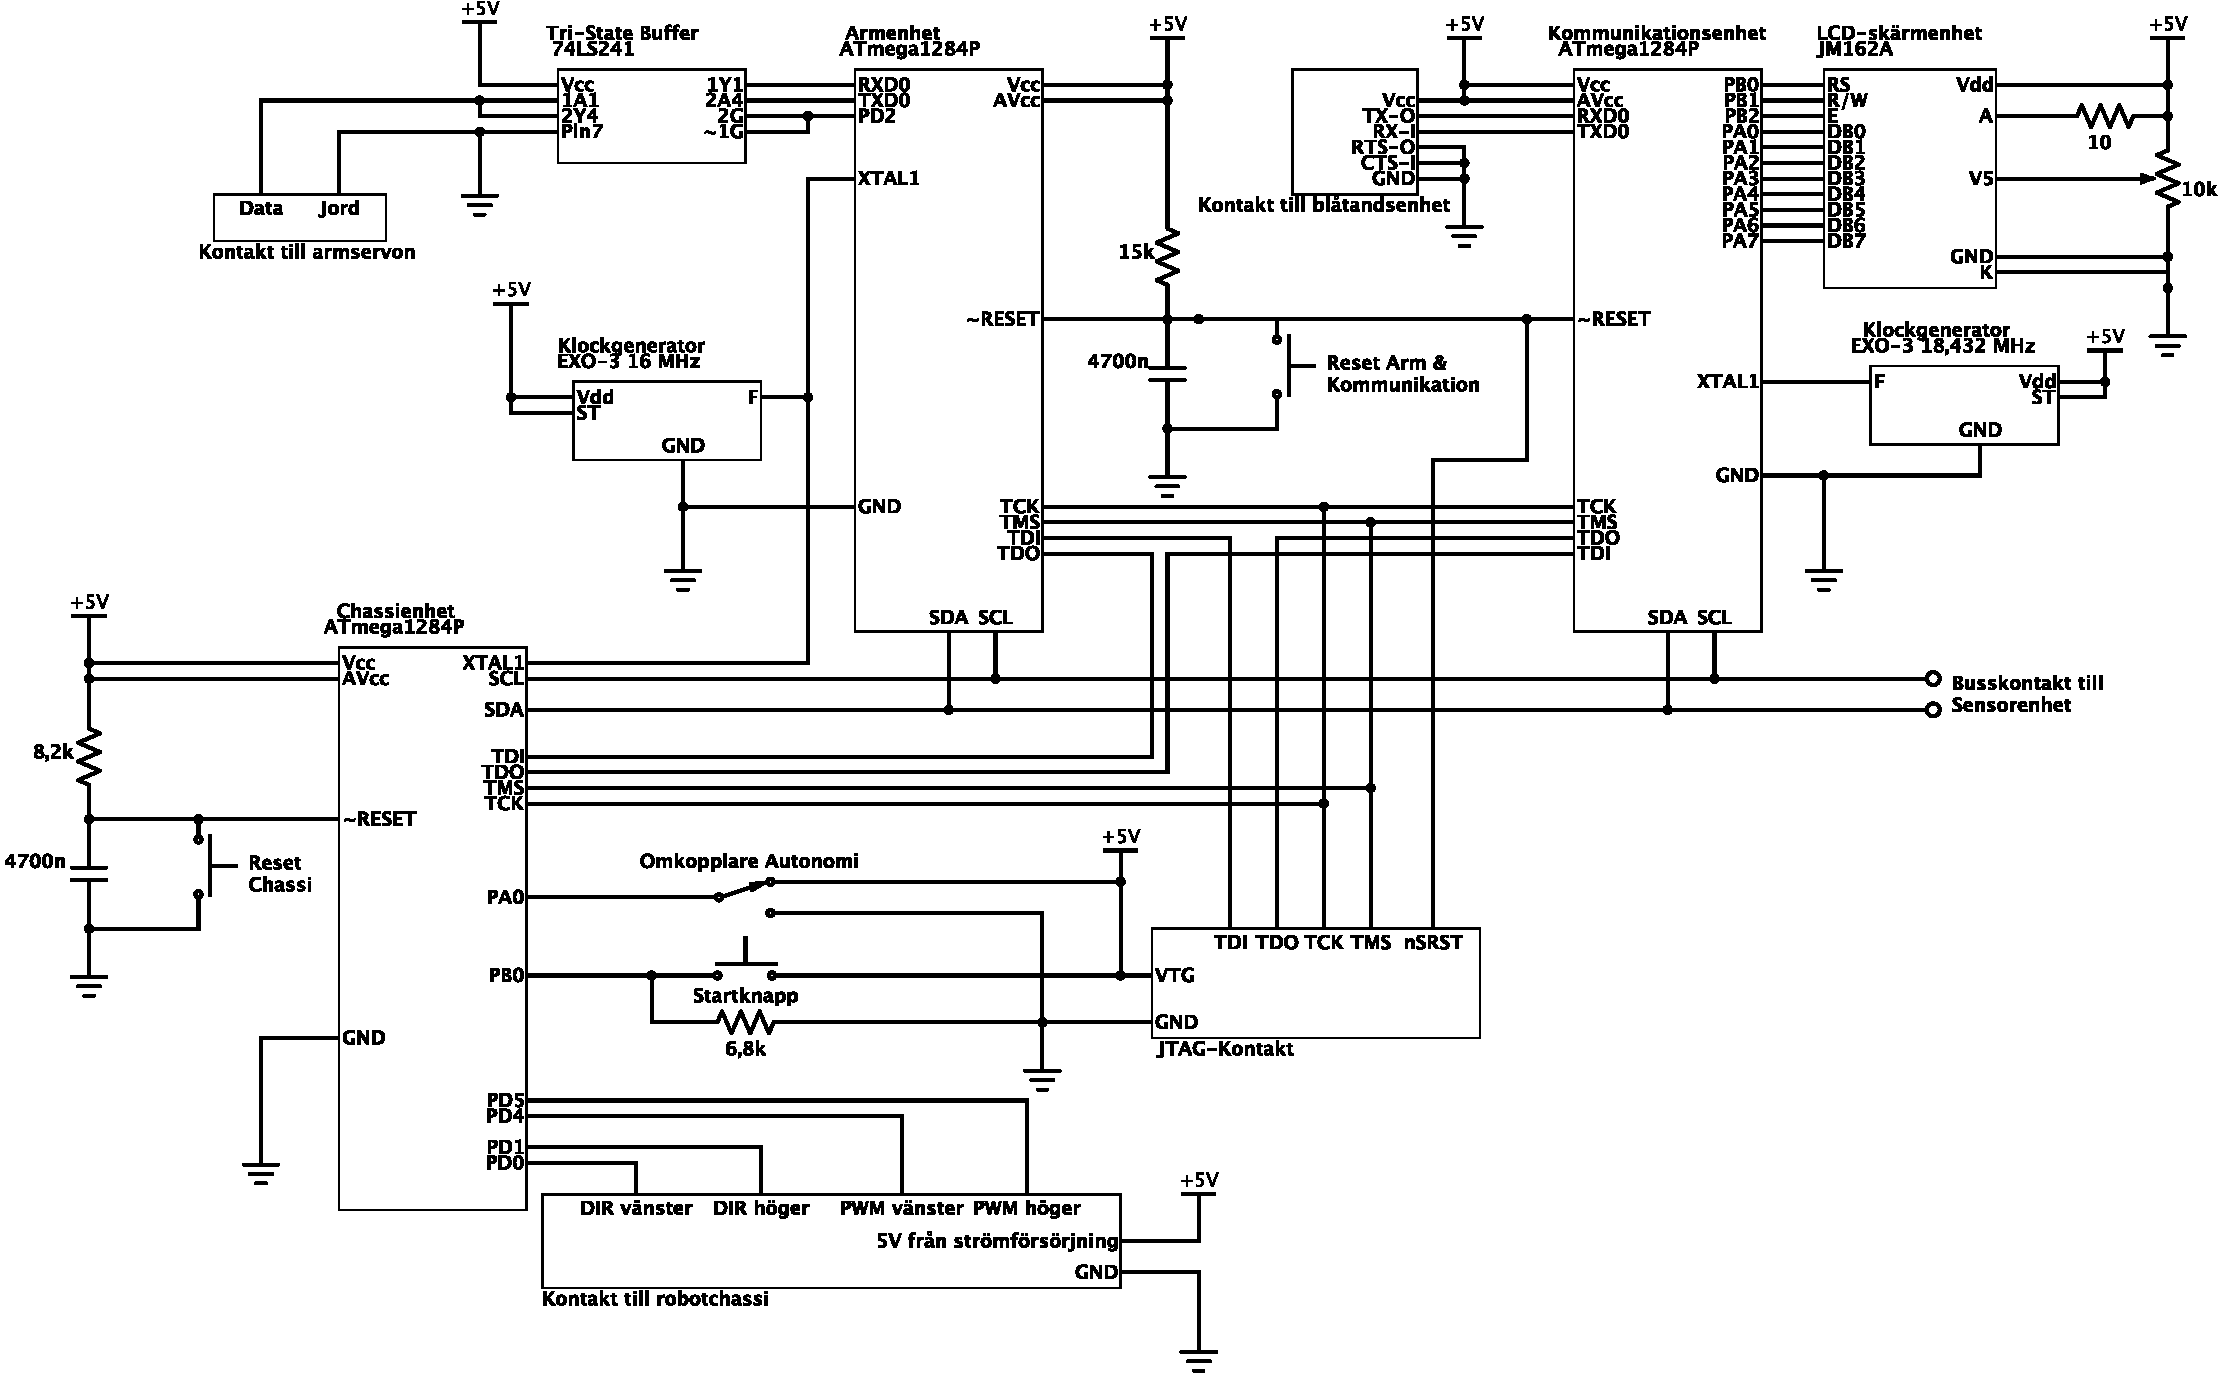
\includegraphics[angle=90,width=0.9\textwidth]{bilder/chassiarmkomm.pdf}
  \emph{\caption{Kopplingsschema över virkortet som innehåller kommunikationsenheten, chassienheten och armenheten.} \label{fig:chassiarmkomm}}
  
\end{figure}


\section{Utdrag från programlistning}
\emph{(ca 5-10 sidor så att vi kan bedöma kodens läsbarhet mm.) och eventuell VHDL-kod}
\section{Övriga bilagor?}


\end{document} 
